\documentclass[11pt, a4paper, notitlepage]{report}
\usepackage[dvips]{graphicx,color,rotating}
\usepackage{polski}
\usepackage[utf8]{inputenc}
\usepackage{pstricks}
\usepackage{lipsum}
\usepackage{titling}
\usepackage{appendix}
\usepackage{hyperref}

\pretitle{
	\begin{center}
		
\includegraphics[width=40pt,height=40pt]{graphics/znak_pk} \\
		 \Huge\bfseries}
\posttitle{\par\end{center}\vskip 0.5em}
\preauthor{\begin{center} \Large  KWD  \\  \LARGE\ttfamily}
\postauthor{ \end{center}}
\predate{\par\large\centering}
\postdate{\par}

\pagestyle{headings}

\author{Krzysztof \textsc{Michalski} \\ Rafał \textsc{Pokrywka} }

\title{\textbf{Neuronowy model dawcy krwi}}
\date{27.01.2020}

\pagenumbering{roman}

\begin{document}
\clearpage\maketitle
\thispagestyle{empty}
\begin{abstract}
	W tym projekcie zajmowaliśmy się przewidywaniem, czy pacjent odda krew w marcu 2007, na podstawie danych z \href{https://archive.ics.uci.edu/ml/datasets/Blood+Transfusion+Service+Center/}{Blood Transfusion Service Center Data Set}.
	Było to zatem zadanie klasyfikacji binarnej. Zastosowaliśmy kilka modeli - regresję liniową, regresję z użyciem drzew decyzyjnych i lasów losowych oraz w pełni połączoną sieć neuronową. Modele zostały poddane analizie skuteczności i na jej podstawie
	najlepszy okazał się \ldots z dokładnością \ldots
\end{abstract}

\clearpage \tableofcontents
\thispagestyle{empty}

\setcounter{page}{1}

\chapter{Wprowadzenie}
\pagenumbering{arabic}
	Dane do projektu uzyskaliśmy ze strony \href{https://archive.ics.uci.edu/ml/datasets/Blood+Transfusion+Service+Center/}{Blood Transfusion Service Center Data Set}. Składały się one z dwóch plików {\it transfusion.data} i {\it transfusion.names}.\\ \\
	W pliku  {\it transfusion.data} znajdowało się 748 przykładów opisanych 4 cechami:
	\begin{itemize}
	  \item R (Recency - months since last donation)
	  \item F (Frequency - total number of donation)
	  \item M (Monetary - total blood donated in c.c.)
	 \item T (Time - months since first donation)
	\end{itemize} oraz jedną etykietą - binary variable representing whether he/she donated blood in March 2007 (1 stand for donating blood; 0 stands for not donating blood). Zatem zadanie można zaliczyć do kategorii klasyfikacji binarnej. Klasy te były słabo zrównoważone - klasę 1
	posiadało około 24\% przykładów, a klasę 0 - 76\%.\\ \\
	W pliku {\it transfusion.names} znajdował się opis danych - źródło, opis atrybutów oraz autorzy.
\section{Opis problemu}
	Zadanie polega na klasyfikacji binarnej przykładów na podstawie 4 cech numerycznych. Celem klasyfikacji, jest określenie, czy nowy pacjent kliniki odda krew po pewnym okresie czasu. W tym celu można wykorzystać różne techniki uczenia maszynowego
	takie jak regresja liniowa, drzewa decyzycjne, lasy losowe czy sieci neuronowe. Ze względu na niewielką ilość przykładów oraz cech je opisujących, skuteczność takiej klasyfikacji może być niewielka - zbiory danych o takiej wielkości są niewystarczające
	dla dobrego wytrenowania na przykład sieci neuronowej. Ze względu na niezrównoważenie klas, modele mogą mieć tendencję do częstszego przewidywania dominującej klasy - bo zapewnia to dużą dokładność takiego modelu. Można spróbować zrównoważyć
	zbiór wybierając podzbiór przykładów o takiej samej reprezentacji klasy pozytywnej i negatywnej.

\chapter{Opis metody}
\section{Wprowadzenie teoretyczne}
	W celu rozwiązania zadania wykorzystaliśmy kilka metod uczenia maszynowego: \\ \\
	{\bf Regresję logistyczną} - czyli metodę służącą do klasyfikacji binarnej, pozwalającą określić prawdopodobieństo przynależności przykładu do jednej z dwóch klas. Jeżeli prawdopodobieństwo to przekracza 50\% oznacza to, że model przewiduje, że dany przykład należy
	do tej klasy. Do nauki regregresora logistycznego wykorzystywana jest:
	\begin{itemize}
	  \item Logarytmiczna funkcja straty, która wykonuje nieliniową transformacje wyjściowych wartości na przedział od 0 do 1, tak, żeby suma wartości obu klas wynosiła 1. 
	  \item Metoda spadku wzdłuż gradientu prostego - pozwalająca zbliżać się do minumum globalnego powyższej funkcji straty.
	  \item Funkcję logistyczną - pozwalającą określić wartość prawdopodobieństwa dla każdej klasy.
	 \end{itemize} 
	{\bf Drzewa decyzyjne} - czyli wszechstronny algorytm uczenia maszynowego, który można wykorzystywać do różnych zadań - zarówno klasyfikacji (binarnej i wieloklasowej) jak i do zadań regresji. Podejście tego modelu do klasyfikacji binarnej polega na
	 dzieleniu każdej z cech danych na dwa zbiory w sposób liniowy - tak, żeby zbiory te były jak najlepiej rozdzielone. Oznacza to, że w podzbiorach przykładów po każdej ze stron tej tak zwanej granicy decyzyjnej, znadowało się jak najwięcej przykładów należących do jednej klasy - 
	 podzbiory te powinien być jak najmniej zanieczyszczone przykładami należącymi do drugiej grupy. Wysokość takiego drzewa określa ile takich liniowych podziałów cech przykładu może wykonać model. \\ \\
	{\bf Lasy losowe} - jest to jedna z metod uczenia zespołowego. Polega ona na wytrenowaniu pewnej ilości drzew decyzyjnych, a następnie zastosowaniu jednej z technik głosowania drzew w celu określenia rezultatu. Głosowanie można przeprowadzać na przykład w sposób
	 większościowy - w takim przypadku, każdy model określa, do której klasy według niego należy dany przykład - klasa określana przez zespół to ta, na którą głosowało najwięcej modeli. \\ \\
	{\bf Sieci neuronowe} - czyli algorytm wielokrotnej zmiany reprezentacji cech określających przykłady, w celu znalezienia reprezentacji pozwalającej - w przypadku klasyfikacji - w jak największym stopniu rozdzielić od siebie przykłady należące do różnych klas. Sieci składają się z:
	\begin{itemize}
	  \item Neuronów - które są elementami wykonującymi liniową transformację danych otrzymywanych na wejściu - sumę ważoną wejść wraz z tak zwanym członem obciążenia, niezależnym od wartości wejść.
	  \item Warstw - które są złożone z neuronów. Neurony w ramach jednej warstwy nie są ze sobą połączone.
	  \item Połączeń pomiedzy warstwami - czyli połączeniem danych wejściowych do neuronów pierwszej warstwy, a następnie wyjść neuronów jednej warstwy z wejściami neuronów kolejnej wastwy.
	 \item Funkcji aktywacji - określających sposób modyfikacji reprezentacji danych przekazywanych pomiędzy warstwami. W przypadku klasyfikacji ostatnia warstwa stosuje funkcję softmax zwracającą prawdopodobieństwa przynależności danego przykładu do danej klasy.
	\end{itemize}
	Sieci neuronowe są trenowane z użyciem metody spadku wzdłuż gradientu prostego. Każdy krok takiej nauki określa się jako epokę danej sieci.
\section{Badania symulacyjne}

Na początku programu, w funkcji load_and_analyze_data, wczytaliśmy zbiór danych i wyświetliliśmy informacje na jego temat.
Żeby zapoznać się z rozkładem danych, sprawdzilismy czy i jakie są korelacje pomiędzy poszczególnymi kolumnami, oraz jakie są minimalne, średnie i maksymalne wartości.

Analiza zbioru danych w wersji niezrównoważonej:
\begin{verbatim}
+----+-----------+-----------+-----------+------------+------------+
|    |         R |         F |         M |          T |          D |
|----+-----------+-----------+-----------+------------+------------|
| R  |  1        | -0.182745 | -0.182745 |  0.160618  | -0.279869  |
| F  | -0.182745 |  1        |  1        |  0.63494   |  0.218633  |
| M  | -0.182745 |  1        |  1        |  0.63494   |  0.218633  |
| T  |  0.160618 |  0.63494  |  0.63494  |  1         | -0.0358544 |
| D  | -0.279869 |  0.218633 |  0.218633 | -0.0358544 |  1         |
+----+-----------+-----------+-----------+------------+------------+

+-------+-----------+-----------+----------+----------+------------+
|       |         R |         F |        M |        T |          D |
|-------+-----------+-----------+----------+----------+------------|
| count | 748       | 748       |   748    | 748      | 748        |
| mean  |   9.50668 |   5.51471 |  1378.68 |  34.2821 |   0.237968 |
| std   |   8.0954  |   5.83931 |  1459.83 |  24.3767 |   0.426124 |
| min   |   0       |   1       |   250    |   2      |   0        |
| 25%   |   2.75    |   2       |   500    |  16      |   0        |
| 50%   |   7       |   4       |  1000    |  28      |   0        |
| 75%   |  14       |   7       |  1750    |  50      |   0        |
| max   |  74       |  50       | 12500    |  98      |   1        |
+-------+-----------+-----------+----------+----------+------------+
\end{verbatim}

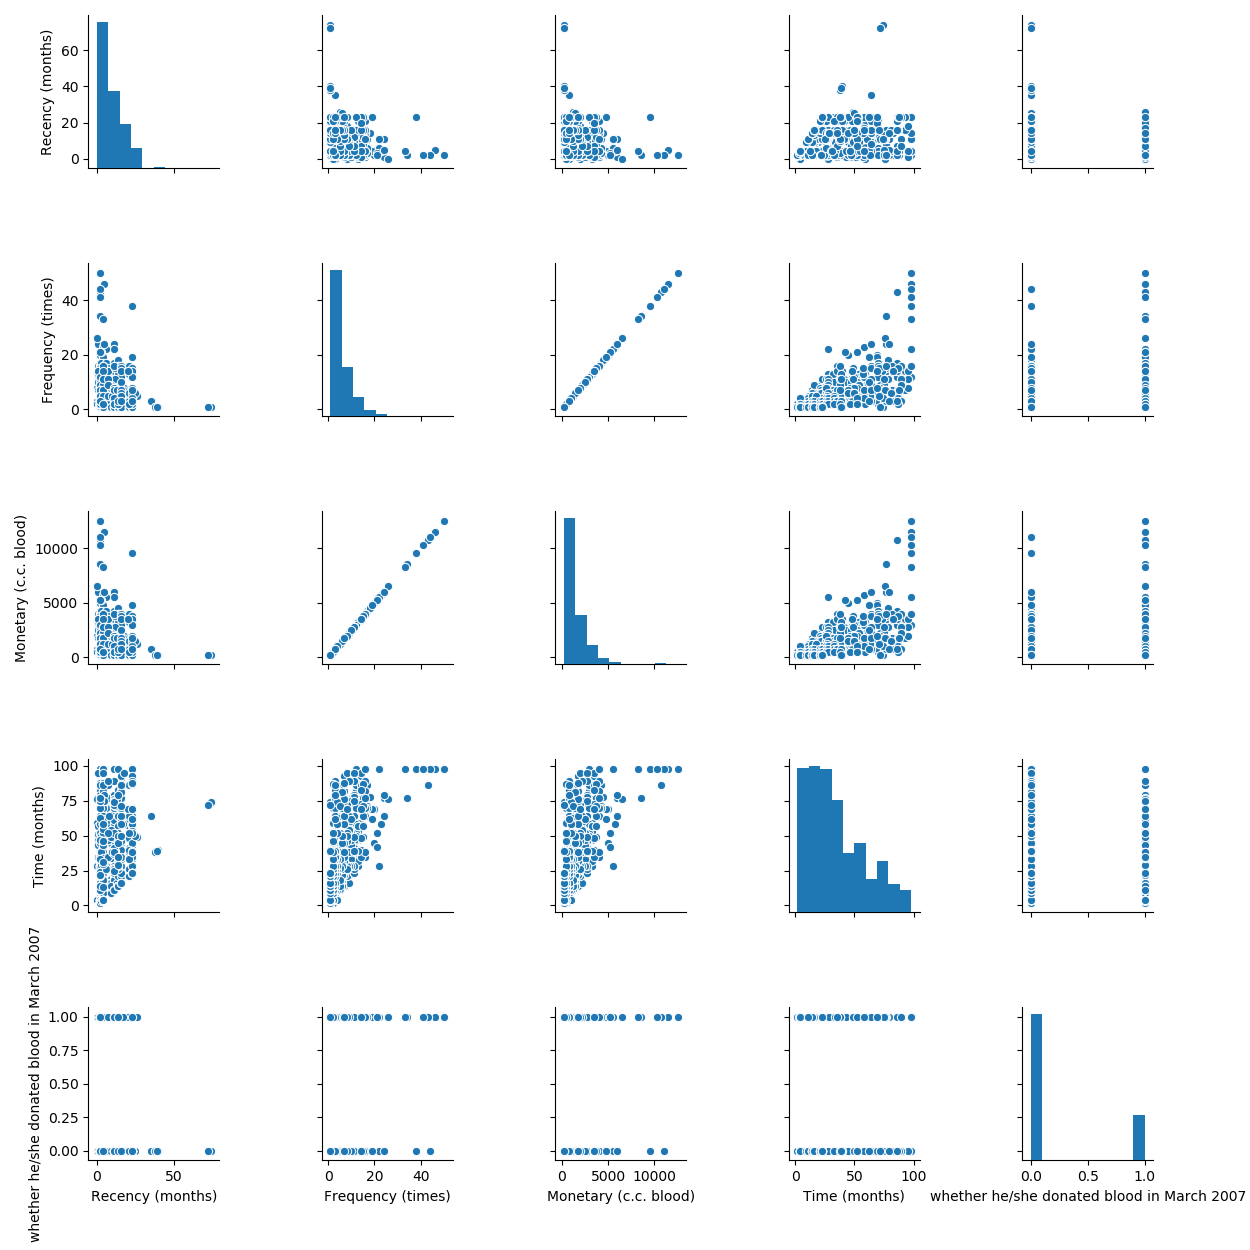
\includegraphics[width=400pt,height=400pt]{graphics/correlation_1} \\

Ponieważ średnia wartość kolumny D (0 lub 1) jest równa 0.237968, to znaczy że tylko ~24\% wierszy ma jedynkę, czyli ilość przykładów dla klas jest niezrównoważona.
Stworzyliśmy więc dodatkowy zbiór danych, który składa się z równej ilości przykładów dla każdej z klas.

Analiza zbioru danych w wersji zrównoważonej:

\begin{verbatim}
+----+------------+-----------+-----------+------------+------------+
|    |          R |         F |         M |          T |          D |
|----+------------+-----------+-----------+------------+------------|
| R  |  1         | -0.218071 | -0.218071 |  0.0949278 | -0.348375  |
| F  | -0.218071  |  1        |  1        |  0.685435  |  0.216987  |
| M  | -0.218071  |  1        |  1        |  0.685435  |  0.216987  |
| T  |  0.0949278 |  0.685435 |  0.685435 |  1         | -0.0152334 |
| D  | -0.348375  |  0.216987 |  0.216987 | -0.0152334 |  1         |
+----+------------+-----------+-----------+------------+------------+

+-------+-----------+-----------+----------+----------+------------+
|       |         R |         F |        M |        T |          D |
|-------+-----------+-----------+----------+----------+------------|
| count | 356       | 356       |   356    | 356      | 356        |
| mean  |   7.95787 |   6.34551 |  1586.38 |  33.0815 |   0.5      |
| std   |   7.19436 |   6.70222 |  1675.55 |  23.8207 |   0.500704 |
| min   |   0       |   1       |   250    |   2      |   0        |
| 25%   |   2       |   2       |   500    |  16      |   0        |
| 50%   |   4       |   5       |  1250    |  28      |   0.5      |
| 75%   |  13.25    |   8       |  2000    |  46      |   1        |
| max   |  40       |  50       | 12500    |  98      |   1        |
+-------+-----------+-----------+----------+----------+------------+
\end{verbatim}

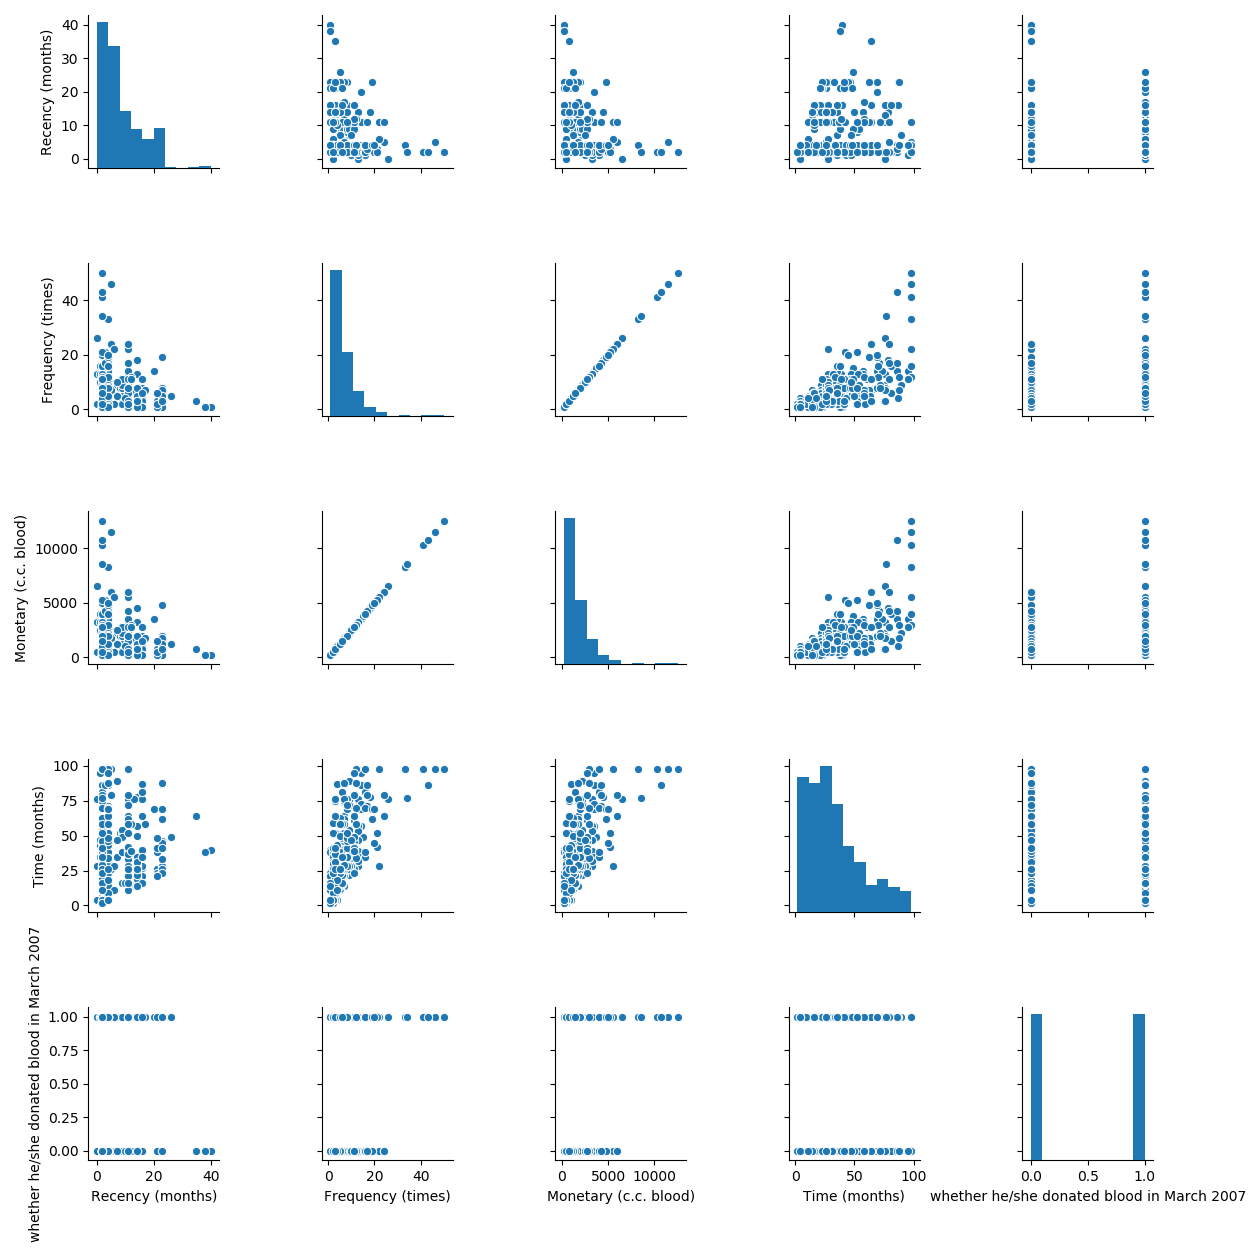
\includegraphics[width=400pt,height=400pt]{graphics/correlation_2} \\

Ponieważ okazało się, że kolumny F i M są ze sobą idealnie skorelowane (F to liczba oddań krwi, a M to suma obiętości oddanej krwi), to możemy pozbyć się jednej z nich, a przewidywania programu nie ulegną zmianie.
Następnie dane należało przeskalować, aby znajdowały się w jednym przedziale wartości, a ich średnia wynosiła zero.
Dzięki temu każda cecha będzie traktowana w równy sposób przez algorytmy uczące.


Gdy dane są już odpowiednio przygotowane, można je podzielić na dwa zbiory: trenujący i testujący.
W naszym programie 90\% to będą dane trenujące, a 10\% testujące.

W celu porównania różnych klasyfikatorów, sprawdzamy w pętli wszystkie podane modele (LogisticRegression, DecisionTreeClassifier, RandomForestClassifier).
Wszystkie te klasyfikatory uczymy z różnymi metaparametrami, np. głębokością drzewa, ilością powtórzeń itp.
Po wyuczeniu każdego z modeli, wypisujemy na wyjście podstawowe informacje o nim (np. dokładność, macierz konfuzji, wykres, ...), oraz .... [KRZYSIEK? POMOCY?].

Później sprawdzamy również jak z tym problemem poradzi sobie sieć neuronowa.
Tworzymy sieć neuronową składającą się z 3 warstw gęstych, mających kolejno 8, 5 i 1 neuronów.
Pierwsze dwie warstwy mają aktywację relu, a ostatnia sigmoid.
Dodatkowo środkowa warstwa ma ustawiony dropout na 10\% - w celu ograniczenia ryzyka przeuczenia sieci.
Metaparametr learning rate ustawiamy na 0.003 - im mniejsza wartość, tym dokładniejsze rozwiązanie można znaleźć, ale jest również ryzyko utknięcia w minimum lokalnym.

Tak utworzoną sieć, zaczynamy uczyć na danych trenujących, z 1000 epok, oraz podając na których danych mają odbywać się testy.
Ponieważ niektóre algorytmy najlepiej się uczą gdy w każdej epoce dane są podawane w innej kolejnści, to ustawiamy również parametr shuffle=True.

Po zakończonym trenowaniu, wypisujemy informacje o efektach:
- jaka jest dokładność przewidywań na zbiorze treningowym, oraz na zbiorze testującym
- jak wygląda macierz konfuzji - żeby zobaczyć jakiego rodzaju błędy najczęściej zostały popełnione (false positives, false negatives)
oraz rysujemy wykresy dokładności w zależności od liczby epok uczenia.

Wszystkie powyższe operacje wykonujemy dla obu zbiorów danych (niezrównoważonego i zrównoważonego).

\chapter{Podsumowanie}
\lipsum[2]


\begin{appendices}
\chapter{Kod programu}
\begin{verbatim}
import numpy as np

a = np.array([1,2])
b =  np.array([1,2])
c =  a + b
print(c) # printing results
\end{verbatim}
\end{appendices}

\end{document}